\documentclass[aspectratio=169, 10pt]{beamer}

% ---------- Tema y colores ----------
\usetheme{default}
\usecolortheme{default}
\setbeamertemplate{navigation symbols}{}
\setbeamertemplate{footline}[frame number]
\setbeamertemplate{frametitle continuation}{}

\definecolor{StanfordRed}{RGB}{140,21,21}
\definecolor{LightGray}{RGB}{240,240,240}
\definecolor{AccentGreen}{RGB}{0,130,100}
\definecolor{UCMBlue}{RGB}{4, 171, 226}
\definecolor{UCMNavy}{RGB}{20, 65, 134}

\definecolor{mitblue}{RGB}{20, 65, 134}
\definecolor{mitgray}{RGB}{169, 169, 169}

\definecolor{AdaptRed}{RGB}{200, 40, 40}
\definecolor{FixedBlue}{RGB}{20, 65, 134}

\setbeamercolor{frametitle}{fg=white, bg=UCMBlue}
\setbeamercolor{title}{fg=white}
\setbeamercolor{author}{fg=white}
\setbeamercolor{institute}{fg=white!80}
\setbeamercolor{structure}{fg=UCMBlue}
\setbeamercolor{block title}{bg=UCMBlue!15!white, fg=UCMBlue}
\setbeamercolor{block body}{bg=LightGray}
\setbeamercolor{block title alerted}{bg=StanfordRed!15!white, fg=StanfordRed}
\setbeamercolor{block body alerted}{bg=LightGray}
\setbeamercolor{alerted text}{fg=UCMBlue}

\setbeamerfont{frametitle}{series=\bfseries, size=\large}
\setbeamerfont{title}{series=\bfseries, size=\LARGE}
\setbeamerfont{block title}{series=\bfseries}

% ---------- Paquetes ----------
\usepackage[utf8]{inputenc}
\usepackage[T1]{fontenc}
\usepackage[provide=*,spanish]{babel}
\usepackage{amsmath, amssymb}
\usepackage{graphicx}
\usepackage{tikz}
\usepackage{pgfplots}
\pgfplotsset{compat=1.18}
\usetikzlibrary{arrows, arrows.meta, shapes, shapes.geometric, positioning,
	fit, calc, matrix, chains, mindmap, decorations.pathreplacing,
	backgrounds, shadows, patterns}
\usepackage{booktabs}
\usepackage{array}
\usepackage{xcolor}
\usepackage{multicol}
\usepackage{tcolorbox}
\tcbuselibrary{skins, breakable}
\usepackage{fontawesome5}

% ---------- Comandos utiles ----------
\providecommand{\R}{\mathbb{R}}
\providecommand{\E}{\mathbb{E}}
\newcommand{\frozen}{{\color{FixedBlue}\faLock}}
\newcommand{\tuned}{{\color{AdaptRed}\faFire}}
\newcommand{\ad}[1]{{\color{AdaptRed}#1}}
\newcommand{\fx}[1]{{\color{FixedBlue}#1}}

\newcommand{\formula}[1]{%
	\begin{tcolorbox}[colback=UCMBlue!8, colframe=UCMBlue, arc=4pt,
		boxsep=2pt, left=6pt, right=6pt, top=3pt, bottom=3pt]
		#1
	\end{tcolorbox}
}

% Cifra destacada (numero grande + descripcion)
\newcommand{\cifra}[2]{%
	\begin{center}
		{\fontsize{30}{32}\selectfont\bfseries\color{UCMNavy}#1}\\[4pt]
		\parbox{0.95\linewidth}{\centering\small #2}
	\end{center}
}

% ---------- Portada ----------
\title{\textbf{Segmentaci\'on Sem\'antica}}
\subtitle{De U-Net a Segment Anything, con aplicaci\'on a la retinopat\'ia diab\'etica}
\author{Sergio Hern\'andez, PhD\\ shernandez@ucm.cl}
\institute{
	\begin{tikzpicture}[scale=0.42, every node/.style={transform shape}]
		\foreach \i/\y in {1/0,2/1,3/2}{\node[circle,draw=white,fill=white!20,minimum size=4mm] (i\i) at (0,\y){};}
		\foreach \i/\y in {1/-0.5,2/0.5,3/1.5,4/2.5}{\node[circle,draw=white,fill=white!35,minimum size=4mm] (h\i) at (2,\y){};}
		\foreach \i/\y in {1/0.5,2/1.5}{\node[circle,draw=white,fill=white!50,minimum size=4mm] (o\i) at (4,\y){};}
		\foreach \a in {1,2,3}\foreach \b in {1,2,3,4}{\draw[white,opacity=0.5] (i\a)--(h\b);}
		\foreach \a in {1,2,3,4}\foreach \b in {1,2}{\draw[white,opacity=0.5] (h\a)--(o\b);}
	\end{tikzpicture}
	\\ \textbf{Mag\'ister en Data Science --- Universidad Cat\'olica del Maule}}
\date{}

\begin{document}
% --- Titulo ---
{
	\setbeamertemplate{background}{
		\begin{tikzpicture}[remember picture, overlay]
			\fill[UCMBlue] (current page.south west) rectangle (current page.north east);
			\fill[UCMBlue!70!black, opacity=0.5]
			(current page.south west) -- ++(0,3) -- ++(18,0) -- cycle;
			\foreach \i in {1,...,40}{
				\fill[white, opacity=0.04]
				({random()*17}, {random()*10}) circle ({random()*0.3});
			}
		\end{tikzpicture}
	}
	\begin{frame}[plain]
		\vspace{1.2cm}
		\titlepage
		\begin{tikzpicture}[remember picture, overlay]
			\node[white, opacity=0.15, font=\fontsize{80}{80}\selectfont]
			at (current page.east) [xshift=-2cm] {$\circlearrowright$};
		\end{tikzpicture}
	\end{frame}
}

\begin{frame}{Hoja de Ruta}
	\tableofcontents
	\note{Cinco bloques. Los tres primeros son el andamiaje cl\'asico que cualquier modelo moderno sigue usando: tareas, m\'etricas, arquitecturas y p\'erdidas. El cuarto introduce el cambio de paradigma de los modelos fundacionales. El quinto aterriza todo en un problema cl\'inico real.}
\end{frame}

% =================================================================
\section{Fundamentos}

\begin{frame}{Segmentaci\'on Sem\'antica vs.\ Clasificaci\'on}
	\begin{figure}
		\centering
		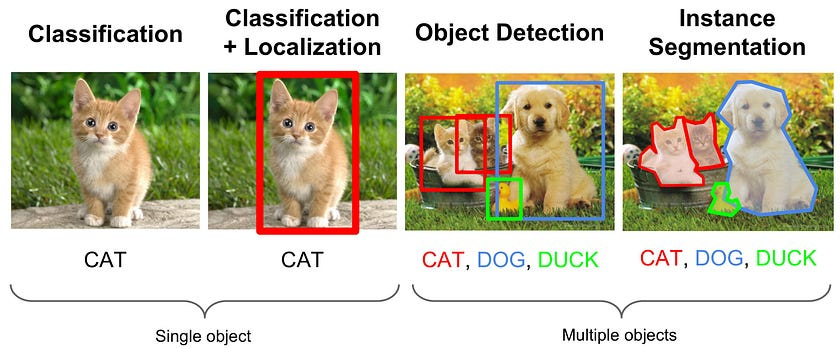
\includegraphics[width=0.8\textwidth, height=0.5\textheight,
		keepaspectratio]{figures/semantic_segmentation_vs_classification}
	\end{figure}

	\begin{columns}[T]
		\begin{column}{0.5\textwidth}
			\begin{block}{Clasificaci\'on}
				\small
				\begin{itemize}
					\item Una etiqueta para \textbf{la imagen completa}.
					\item Responde: \textit{?`qu\'e es esto?}
					\item Salida: clase global y probabilidades.
				\end{itemize}
			\end{block}
		\end{column}

		\begin{column}{0.5\textwidth}
			\begin{block}{Segmentaci\'on Sem\'antica}
				\small
				\begin{itemize}
					\item Una etiqueta para \textbf{cada pixel}.
					\item Responde: \textit{?`qu\'e es cada parte?}
					\item Salida: mapa de etiquetas (alto $\times$ ancho).
				\end{itemize}
			\end{block}
		\end{column}
	\end{columns}

	\note{Punto de partida: la clasificaci\'on responde qu\'e hay en la imagen; la segmentaci\'on responde d\'onde est\'a cada cosa, pixel a pixel.}
\end{frame}

\begin{frame}{Tres Formas de Segmentar una Imagen}

	\formula{
		\[
		f : \R^{H \times W \times 3} \to \{1, \dots, K\}^{H \times W}
		\qquad \text{(asignar una de $K$ clases a cada pixel)}
		\]
	}

	\begin{columns}[T]
		\begin{column}{0.33\textwidth}
			\begin{block}{Sem\'antica}
				\small
				Una etiqueta por pixel. Dos personas forman una sola regi\'on ``persona''.

				\textbf{Ej.:} FCN, U-Net, DeepLab.
			\end{block}
		\end{column}

		\begin{column}{0.33\textwidth}
			\begin{block}{Instancia}
				\small
				Cada objeto de una misma clase recibe su propia m\'ascara.

				\textbf{Ej.:} Mask R-CNN.
			\end{block}
		\end{column}

		\begin{column}{0.33\textwidth}
			\begin{block}{Pan\'optica}
				\small
				Une ambas: regiones amorfas (cielo, pista) y objetos contables con identidad.

				\textbf{Ej.:} Mask2Former.
			\end{block}
		\end{column}
	\end{columns}

	\vspace{0.2cm}

	\begin{alertblock}{Ojo}
		SAM no hace ninguna de las tres exactamente: produce m\'ascaras \textbf{sin clase} a partir de un prompt.
	\end{alertblock}

	\note{Definici\'on formal: una funci\'on que mapea la imagen a un mapa de etiquetas del mismo tama\~no. En retinopat\'ia diab\'etica el problema es sem\'antico (qu\'e pixeles son exudado, hemorragia, etc.), no de instancias.}
\end{frame}

\begin{frame}{C\'omo Medimos una M\'ascara}

	\begin{columns}[T]
		\begin{column}{0.33\textwidth}
			\begin{block}{IoU (Jaccard)}
				\small
				\[
				\text{IoU} = \frac{|A \cap B|}{|A \cup B|}
				\]
				Penaliza por igual FP y FN. La mIoU promedia por clase.
			\end{block}
		\end{column}

		\begin{column}{0.33\textwidth}
			\begin{block}{Dice (F1)}
				\small
				\[
				\text{Dice} = \frac{2|A \cap B|}{|A| + |B|}
				\]
				Es el F1 por pixel: $\text{Dice} = \frac{2\,\text{IoU}}{1 + \text{IoU}}$.
			\end{block}
		\end{column}

		\begin{column}{0.33\textwidth}
			\begin{block}{Exactitud de pixel}
				\small
				\[
				\text{Acc} = \frac{\text{correctos}}{\text{total}}
				\]
				Enga\~nosa con desbalance: si la lesi\'on ocupa menos del 1\%, predecir ``fondo'' en todo da m\'as de 99\%.
			\end{block}
		\end{column}
	\end{columns}

	\vspace{0.3cm}

	\begin{alertblock}{En video}
		SAM 2 reporta $\mathcal{J}\&\mathcal{F}$: $\mathcal{J}$ es la IoU de la regi\'on y $\mathcal{F}$ la precisi\'on del contorno.
	\end{alertblock}

	\note{A es la predicci\'on y B el ground truth. Pedir a los estudiantes que demuestren Dice = 2 IoU/(1+IoU): ambas m\'etricas ordenan igual a los modelos, pero Dice es m\'as generosa. La exactitud de pixel es el error cl\'asico en im\'agenes m\'edicas.}
\end{frame}

% =================================================================
\section{Arquitecturas Cl\'asicas}

\begin{frame}{Una D\'ecada de Segmentaci\'on con Deep Learning}

	\vspace{0.4cm}

	\begin{center}
		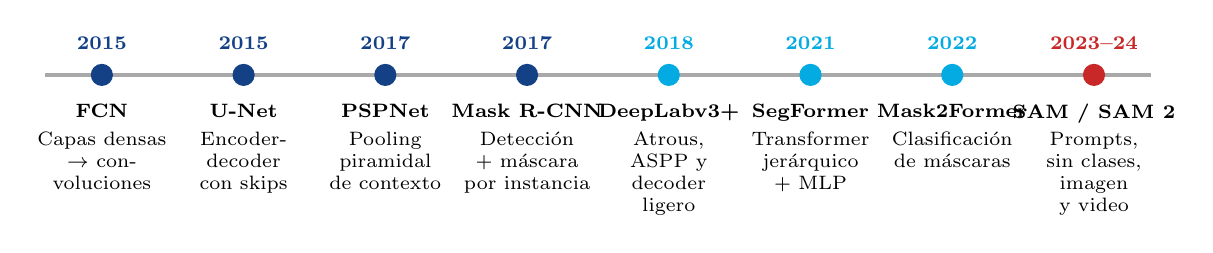
\begin{tikzpicture}[x=1.8cm,
				yr/.style={font=\scriptsize\bfseries, anchor=south},
				nm/.style={font=\scriptsize\bfseries, anchor=north},
				ds/.style={font=\scriptsize, anchor=north, text width=1.65cm, align=center}]
			\draw[very thick, mitgray] (-0.4,0) -- (7.4,0);

			\foreach \x/\c in {0/UCMNavy,1/UCMNavy,2/UCMNavy,3/UCMNavy,4/UCMBlue,5/UCMBlue,6/UCMBlue,7/AdaptRed}{
				\fill[\c] (\x,0) circle (4pt);
			}

			\node[yr, UCMNavy] at (0,0.2) {2015}; \node[nm] at (0,-0.25) {FCN};
			\node[ds] at (0,-0.6) {Capas densas $\to$ convoluciones};

			\node[yr, UCMNavy] at (1,0.2) {2015}; \node[nm] at (1,-0.25) {U-Net};
			\node[ds] at (1,-0.6) {Encoder-decoder con skips};

			\node[yr, UCMNavy] at (2,0.2) {2017}; \node[nm] at (2,-0.25) {PSPNet};
			\node[ds] at (2,-0.6) {Pooling piramidal de contexto};

			\node[yr, UCMNavy] at (3,0.2) {2017}; \node[nm] at (3,-0.25) {Mask R-CNN};
			\node[ds] at (3,-0.6) {Detecci\'on + m\'ascara por instancia};

			\node[yr, UCMBlue] at (4,0.2) {2018}; \node[nm] at (4,-0.25) {DeepLabv3+};
			\node[ds] at (4,-0.6) {Atrous, ASPP y decoder ligero};

			\node[yr, UCMBlue] at (5,0.2) {2021}; \node[nm] at (5,-0.25) {SegFormer};
			\node[ds] at (5,-0.6) {Transformer jer\'arquico + MLP};

			\node[yr, UCMBlue] at (6,0.2) {2022}; \node[nm] at (6,-0.25) {Mask2Former};
			\node[ds] at (6,-0.6) {Clasificaci\'on de m\'ascaras};

			\node[yr, AdaptRed] at (7,0.2) {2023--24}; \node[nm] at (7,-0.25) {SAM / SAM 2};
			\node[ds] at (7,-0.6) {Prompts, sin clases, imagen y video};
		\end{tikzpicture}
	\end{center}

	\vspace{0.4cm}

	\begin{block}{Pregunta gu\'ia del bloque}
		?`C\'omo recuperar la resoluci\'on espacial sin perder contexto? Cada arquitectura responde de manera distinta.
	\end{block}

	\note{Tres colores: azul oscuro para la era convolucional fundacional (2015-2017), celeste para la consolidaci\'on y la llegada de los transformers, y rojo para los modelos fundacionales.}
\end{frame}

\begin{frame}{FCN: Clasificar Cada Pixel}

	\textbf{FCN} (Long et al., 2015) reutiliza un clasificador de im\'agenes como clasificador de pixeles.

	\vspace{0.2cm}

	\begin{columns}[c]
		\begin{column}{0.52\textwidth}
			\begin{block}{Tres ideas}
				\small
				\begin{itemize}
					\item \textbf{Convolucionalizar:} las capas densas de VGG se reemplazan por convoluciones $1 \times 1$; acepta cualquier tama\~no.
					\item \textbf{Sobremuestrear:} convoluciones transpuestas recuperan la resoluci\'on que el pooling redujo 32 veces.
					\item \textbf{Saltos:} fusionar capas intermedias (FCN-16s, FCN-8s) devuelve el detalle fino.
				\end{itemize}
			\end{block}
		\end{column}

		\begin{column}{0.46\textwidth}
			\begin{center}
				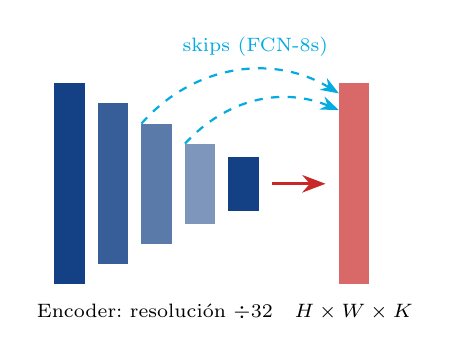
\begin{tikzpicture}[scale=0.85]
					\fill[FixedBlue] (0,-1.5) rectangle (0.45,1.5);
					\fill[FixedBlue!85] (0.65,-1.2) rectangle (1.1,1.2);
					\fill[FixedBlue!70] (1.3,-0.9) rectangle (1.75,0.9);
					\fill[FixedBlue!55] (1.95,-0.6) rectangle (2.4,0.6);
					\fill[UCMNavy] (2.6,-0.4) rectangle (3.05,0.4);
					\draw[-Stealth, very thick, AdaptRed] (3.25,0) -- (4.05,0);
					\fill[AdaptRed!70] (4.25,-1.5) rectangle (4.7,1.5);
					\draw[-Stealth, dashed, UCMBlue, thick] (1.95,0.6) to[bend left=35] (4.25,1.1);
					\draw[-Stealth, dashed, UCMBlue, thick] (1.3,0.9) to[bend left=40] (4.25,1.35);
					\node[font=\scriptsize, anchor=north] at (1.5,-1.65) {Encoder: resoluci\'on $\div 32$};
					\node[font=\scriptsize, anchor=north] at (4.47,-1.65) {$H \times W \times K$};
					\node[font=\scriptsize, UCMBlue] at (3.0,2.05) {skips (FCN-8s)};
				\end{tikzpicture}
			\end{center}
		\end{column}
	\end{columns}

	\note{FCN es el punto de partida conceptual. Su debilidad es que el sobremuestreo desde 1/32 de resoluci\'on produce bordes gruesos; las conexiones de salto mitigan esto y anticipan la idea central de U-Net.}
\end{frame}

\begin{frame}{U-Net: Simetr\'ia y Conexiones de Salto}

	\begin{columns}[c]
		\begin{column}{0.6\textwidth}
			\begin{center}
				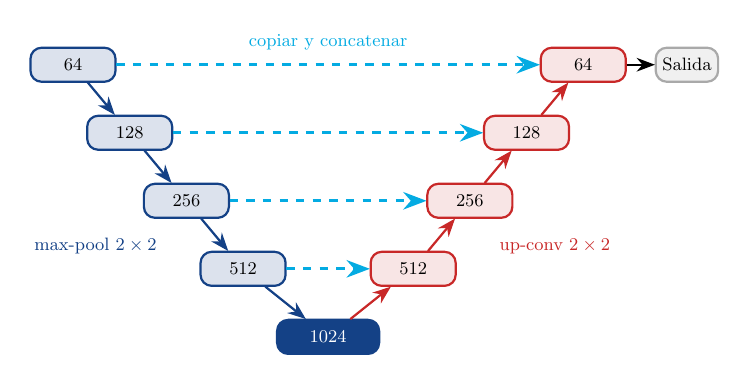
\begin{tikzpicture}[scale=0.72, every node/.style={transform shape},
						enc/.style={draw=FixedBlue, fill=FixedBlue!15, thick, rounded corners, minimum width=1.5cm, minimum height=0.6cm, font=\small},
						dec/.style={draw=AdaptRed, fill=AdaptRed!12, thick, rounded corners, minimum width=1.5cm, minimum height=0.6cm, font=\small},
						arr/.style={-Stealth, thick}]
					\node[enc] (e1) at (0,0) {64};
					\node[enc] (e2) at (1,-1.2) {128};
					\node[enc] (e3) at (2,-2.4) {256};
					\node[enc] (e4) at (3,-3.6) {512};
					\node[draw=UCMNavy, fill=UCMNavy, text=white, thick, rounded corners, minimum width=1.8cm, minimum height=0.6cm, font=\small] (b) at (4.5,-4.8) {1024};
					\node[dec] (d4) at (6,-3.6) {512};
					\node[dec] (d3) at (7,-2.4) {256};
					\node[dec] (d2) at (8,-1.2) {128};
					\node[dec] (d1) at (9,0) {64};
					\node[draw=mitgray, fill=LightGray, thick, rounded corners, minimum height=0.6cm, font=\small, right=0.5cm of d1] (out) {Salida};

					\draw[arr, FixedBlue] (e1) -- (e2); \draw[arr, FixedBlue] (e2) -- (e3);
					\draw[arr, FixedBlue] (e3) -- (e4); \draw[arr, FixedBlue] (e4) -- (b);
					\draw[arr, AdaptRed] (b) -- (d4); \draw[arr, AdaptRed] (d4) -- (d3);
					\draw[arr, AdaptRed] (d3) -- (d2); \draw[arr, AdaptRed] (d2) -- (d1);
					\draw[arr] (d1) -- (out);

					\foreach \k in {1,2,3,4}{\draw[-Stealth, dashed, UCMBlue, very thick] (e\k) -- (d\k);}

					\node[font=\small, FixedBlue, anchor=east] at (1.6,-3.2) {max-pool $2\times2$};
					\node[font=\small, AdaptRed, anchor=west] at (7.4,-3.2) {up-conv $2\times2$};
					\node[font=\small, UCMBlue] at (4.5,0.4) {copiar y concatenar};
				\end{tikzpicture}
			\end{center}
		\end{column}

		\begin{column}{0.38\textwidth}
			\begin{block}{Ronneberger et al., 2015}
				\small
				\begin{itemize}
					\item \textbf{Bajada:} conv $3\times3$ + max-pool; duplica canales, reduce resoluci\'on.
					\item \textbf{Subida:} up-conv y concatenaci\'on con el mapa del mismo nivel.
					\item \textbf{Por qu\'e perdura:} rinde con pocas im\'agenes anotadas; sigue siendo la l\'inea base en imagen m\'edica (nnU-Net).
				\end{itemize}
			\end{block}
		\end{column}
	\end{columns}

	\note{U-Net fue propuesta para microscop\'ia celular con muy pocos datos. El codificador sabe d\'onde, el decodificador sabe qu\'e. nnU-Net (Isensee et al., 2021) mostr\'o que una U-Net bien configurada sigue siendo dif\'icil de superar en desaf\'ios m\'edicos. Ser\'a el baseline del caso de retinopat\'ia.}
\end{frame}

\begin{frame}{U-Net (2015): Diagrama de la Arquitectura}

	\begin{center}
		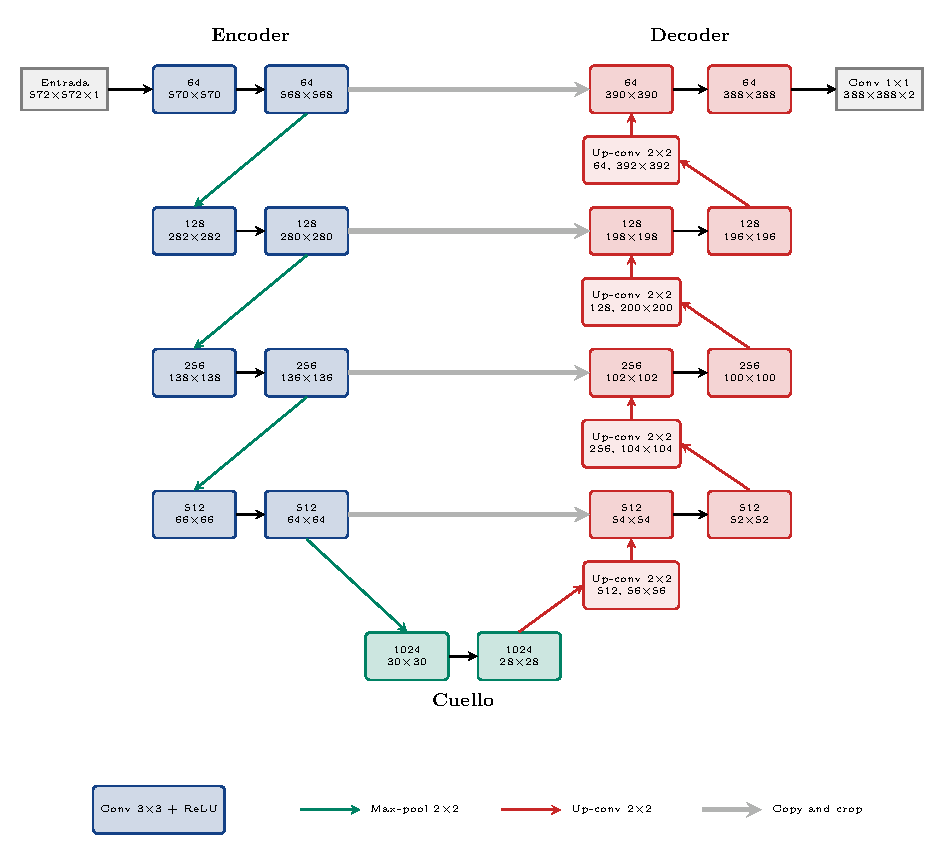
\includegraphics[width=0.85\textwidth, height=\textheight]{architectures/unet_architecture}
	\end{center}

	\note{Diagrama detallado: en el original, las convoluciones no usan padding, por eso el mapa del codificador se recorta antes de concatenar (copy and crop).}
\end{frame}

\begin{frame}{SegNet: Pooling con \'Indices}

	SegNet (Badrinarayanan et al., 2017) almacena solo los \'indices del max-pooling en el encoder y los reutiliza para el unpooling en el decoder.

	\vspace{0.2cm}

	\begin{center}
		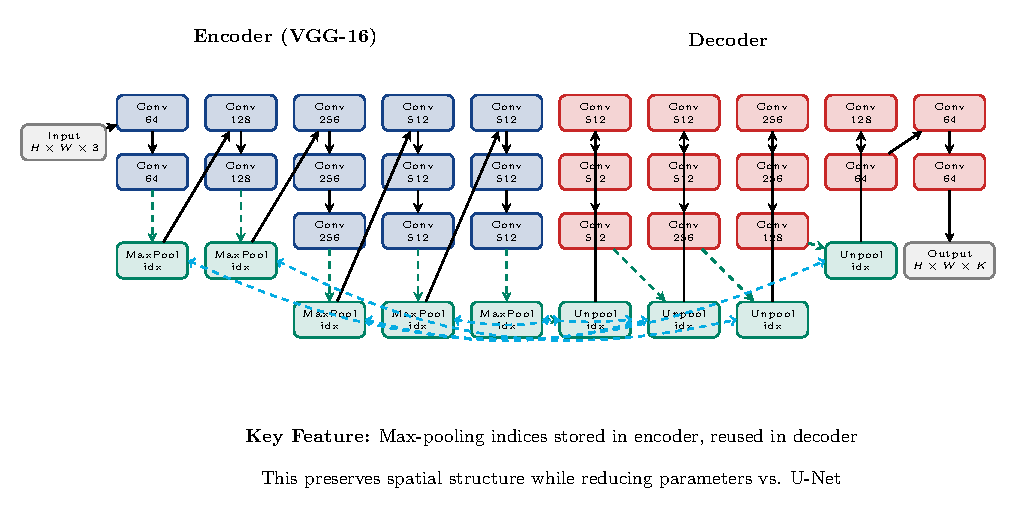
\includegraphics[width=0.92\textwidth, height=0.68\textheight, keepaspectratio]{architectures/segnet_architecture}
	\end{center}

	\note{Contraste con U-Net: SegNet no concatena mapas completos del codificador, solo transfiere los \'indices del max-pooling. Es m\'as liviano en memoria, pero recupera menos detalle fino. El laboratorio 2.6 implementa ambas.}
\end{frame}

\begin{frame}{DeepLab: M\'as Contexto sin Perder Resoluci\'on}

	\textbf{DeepLab} (Chen et al., 2018) usa convoluci\'on atrous (dilatada):

	\formula{
		\[
		y[i] = \sum_{k} x[i + r \cdot k] \cdot w[k], \qquad \text{un filtro } 3 \times 3 \text{ cubre } (2r+1) \times (2r+1) \text{ pixeles}
		\]
	}

	\begin{columns}[c]
		\begin{column}{0.55\textwidth}
			\begin{center}
				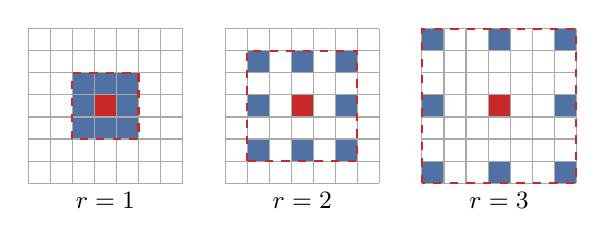
\begin{tikzpicture}
					\foreach \r/\ox in {1/0,2/2.5,3/5}{
						\begin{scope}[shift={(\ox,0)}]
							\fill[white] (0,0) rectangle (1.96,1.96);
							\foreach \i in {-1,0,1}{\foreach \j in {-1,0,1}{
								\fill[FixedBlue!75] ({(3+\i*\r)*0.28},{(3+\j*\r)*0.28}) rectangle ++(0.28,0.28);
							}}
							\fill[AdaptRed] (0.84,0.84) rectangle ++(0.28,0.28);
							\draw[step=0.28, mitgray, thin] (0,0) grid (1.96,1.96);
							\draw[AdaptRed, thick, dashed] ({(3-\r)*0.28},{(3-\r)*0.28}) rectangle ++({(2*\r+1)*0.28},{(2*\r+1)*0.28});
							\node[below, font=\small] at (0.98,0) {$r=\r$};
						\end{scope}
					}
				\end{tikzpicture}
			\end{center}
		\end{column}

		\begin{column}{0.43\textwidth}
			\begin{block}{ASPP}
				\small
				Ramas paralelas con $r = 6, 12, 18$ + pooling global, concatenadas: contexto multiescala.

				\textbf{v1--v2} refinaban con un CRF denso; \textbf{v3+} usa un decoder con features de bajo nivel.
			\end{block}
		\end{column}
	\end{columns}

	\vspace{0.2cm}

	\begin{alertblock}{Ventaja Clave}
		Mayor receptive field sin par\'ametros extra ni reducir resoluci\'on.
	\end{alertblock}

	\note{Las grillas muestran el mismo filtro de 9 pesos (azul y rojo) cubriendo campos de 3, 5 y 7 pixeles. Ojo con el efecto gridding: con tasas grandes quedan huecos sin observar; por eso ASPP combina varias tasas.}
\end{frame}

\begin{frame}{DeepLab: M\'odulo ASPP}

	\begin{center}
		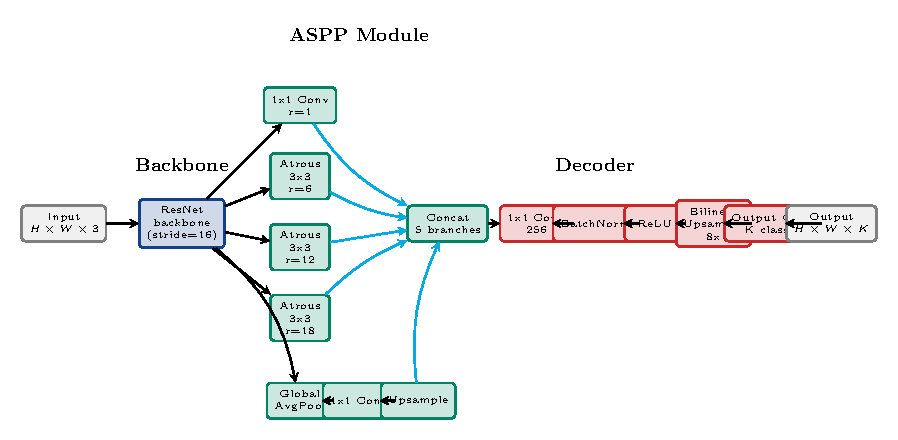
\includegraphics[width=\textwidth, height=\textheight]{architectures/deeplab_aspp}
	\end{center}

	\note{ASPP aplica en paralelo convoluciones dilatadas con distintas tasas y un pooling global, y concatena las salidas antes de proyectarlas con una convoluci\'on 1x1.}
\end{frame}

\begin{frame}{Transformers: de Clasificar Pixeles a Clasificar M\'ascaras}

	\begin{columns}[T]
		\begin{column}{0.33\textwidth}
			\begin{block}{SETR (2021)}
				\small
				Un ViT como codificador: atenci\'on global desde la primera capa, pero costoso en alta resoluci\'on.
			\end{block}
		\end{column}

		\begin{column}{0.33\textwidth}
			\begin{block}{SegFormer (2021)}
				\small
				Codificador jer\'arquico multiescala sin codificaci\'on posicional fija y un decoder MLP ligero.
			\end{block}
		\end{column}

		\begin{column}{0.33\textwidth}
			\begin{block}{Mask2Former (2022)}
				\small
				Predice $N$ m\'ascaras, cada una con su clase, mediante atenci\'on enmascarada. Un modelo para las tres tareas.
			\end{block}
		\end{column}
	\end{columns}

	\vspace{0.4cm}

	\begin{alertblock}{Conexi\'on con SAM}
		SAM hereda esta idea: su decodificador produce \textbf{m\'ascaras}, no un mapa de clases.
	\end{alertblock}

	\note{El cambio conceptual es de clasificaci\'on por pixel a clasificaci\'on de m\'ascaras. SAM lleva la idea al extremo: produce m\'ascaras de calidad sin decidir la clase; la clase queda en manos de quien hace el prompt o de otro modelo.}
\end{frame}

% =================================================================
\section{Funciones Objetivo}

\begin{frame}{P\'erdidas por Pixel: Cross-Entropy y Variantes}

	\begin{block}{Entrop\'ia cruzada (CE)}
		\small
		\[
		\mathcal{L}_{\text{CE}} = -\frac{1}{N} \sum_{i} \sum_{c} y_{ic} \log p_{ic}
		\]
		Cada pixel es una clasificaci\'on independiente; la clase mayoritaria domina el gradiente.
	\end{block}

	\begin{columns}[T]
		\begin{column}{0.5\textwidth}
			\begin{block}{CE ponderada}
				\small
				\[
				\mathcal{L}_{\text{wCE}} = -\frac{1}{N} \sum_{i} \sum_{c} w_c\, y_{ic} \log p_{ic}
				\]
				$w_c \propto 1/\text{frecuencia}$. Compensa el desbalance, pero puede volver ruidoso el entrenamiento.
			\end{block}
		\end{column}

		\begin{column}{0.5\textwidth}
			\begin{block}{Focal (Lin et al., 2017)}
				\small
				\[
				\mathcal{L}_{\text{FL}} = -\alpha\, (1 - p_t)^{\gamma} \log p_t
				\]
				Reduce el peso de los pixeles f\'aciles; $\gamma = 2$ es lo habitual.
			\end{block}
		\end{column}
	\end{columns}

	\note{p_t es la probabilidad asignada a la clase correcta. Intuici\'on de la focal: si el modelo ya acierta con p_t = 0,9, el factor (1-p_t)^2 = 0,01 casi anula esa contribuci\'on; el gradiente se concentra en los pixeles dif\'iciles, t\'ipicamente bordes y lesiones peque\~nas.}
\end{frame}

\begin{frame}{P\'erdidas por Regi\'on: Optimizar el Solapamiento}

	\formula{
		\[
		\mathcal{L}_{\text{Dice}} = 1 - \frac{2 \sum_i p_i g_i + \varepsilon}{\sum_i p_i + \sum_i g_i + \varepsilon}
		\qquad \text{(Milletari et al., 2016)}
		\]
	}

	\begin{columns}[T]
		\begin{column}{0.5\textwidth}
			\begin{block}{Tversky (Salehi et al., 2017)}
				\small
				\[
				\text{TI} = \frac{\text{TP}}{\text{TP} + \alpha\, \text{FP} + \beta\, \text{FN}}
				\]
				Con $\beta > \alpha$ castiga m\'as los falsos negativos. Con $\alpha = \beta = 0{,}5$ recupera Dice.
			\end{block}
		\end{column}

		\begin{column}{0.5\textwidth}
			\begin{block}{Combinada}
				\small
				\[
				\mathcal{L} = \lambda_1 \mathcal{L}_{\text{Focal}} + \lambda_2 \mathcal{L}_{\text{Dice}}
				\]
				Gradientes estables por pixel + objetivo de solapamiento.
			\end{block}
		\end{column}
	\end{columns}

	\vspace{0.2cm}

	\begin{alertblock}{Dato de SAM 2}
		SAM 2 combina focal y Dice en raz\'on 20:1 (m\'as MAE para la IoU predicha y CE para la oclusi\'on).
	\end{alertblock}

	\note{p son probabilidades predichas, g el ground truth binario, epsilon un suavizado. Dice optimiza algo cercano a la m\'etrica de evaluaci\'on, pero es inestable si la lesi\'on es diminuta o no existe. El dato de SAM 2 viene del ap\'endice D.2.2 del paper: raz\'on 20:1:1:1.}
\end{frame}

\begin{frame}{?`Qu\'e P\'erdida Usar?}

	\vspace{0.3cm}

	\begin{center}
		\begin{tabular}{>{\raggedright\arraybackslash}p{4.2cm} >{\raggedright\arraybackslash}p{3.6cm} >{\raggedright\arraybackslash}p{5.2cm}}
			\toprule
			\textbf{Situaci\'on} & \textbf{P\'erdida sugerida} & \textbf{Por qu\'e} \\
			\midrule
			Clases balanceadas, objetos grandes & Entrop\'ia cruzada & Simple y con gradientes estables \\
			Desbalance moderado & CE ponderada & Sube el peso de las clases raras \\
			Objetos peque\~nos o raros & Dice + Focal & Solapamiento sin ahogarse en el fondo \\
			Cribado: no omitir lesiones & Tversky ($\beta > \alpha$) & Prioriza la sensibilidad \\
			Los bordes importan & Boundary loss o Lov\'asz & Supervisa el contorno u optimiza la IoU \\
			\bottomrule
		\end{tabular}
	\end{center}

	\vspace{0.3cm}

	\begin{alertblock}{Estrategia Pr\'actica}
		Empezar con CE (o Focal) + Dice y ajustar solo si la m\'etrica de inter\'es lo pide. En retinopat\'ia diab\'etica estamos en la fila de objetos peque\~nos y raros.
	\end{alertblock}

	\note{Boundary loss: Kervadec et al., 2019. Lov\'asz-Softmax: Berman et al., 2018. Si el objetivo es cribado, tambi\'en aplica la fila de sensibilidad.}
\end{frame}

% =================================================================
\section{Segment Anything}

\begin{frame}{Segment Anything: un Modelo para Cualquier Objeto}

	\textbf{SAM} (Kirillov et al., 2023) define una tarea general, la \textbf{segmentaci\'on por prompts}, y un modelo que la resuelve en cero disparos.

	\vspace{0.4cm}

	\begin{columns}[T]
		\begin{column}{0.33\textwidth}
			\cifra{11\,M}{im\'agenes en el dataset SA-1B}
		\end{column}
		\begin{column}{0.33\textwidth}
			\cifra{1{,}1\,B}{m\'ascaras, anotadas con el modelo en el ciclo}
		\end{column}
		\begin{column}{0.33\textwidth}
			\cifra{3}{tipos de prompt: puntos, cajas y m\'ascaras}
		\end{column}
	\end{columns}

	\vspace{0.3cm}

	\begin{block}{Data engine}
		El modelo ayuda a anotar, los datos mejoran el modelo, y as\'i iterativamente. SAM \textbf{no asigna clases}: devuelve la m\'ascara de lo que el usuario se\~nala.
	\end{block}

	\note{Cambio de paradigma: en vez de entrenar un modelo por tarea y por conjunto de clases, un \'unico modelo promptable que generaliza a dominios nuevos.}
\end{frame}

\begin{frame}{SAM: Codificar una Vez, Decodificar Muchas}

	\begin{center}
		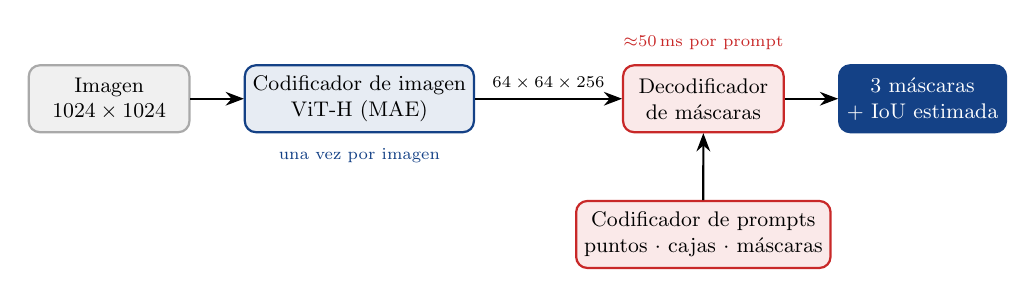
\begin{tikzpicture}[scale=0.85, every node/.style={transform shape},
				lay/.style={draw, thick, rounded corners, minimum width=2.4cm, minimum height=1.0cm, font=\small, align=center},
				arr/.style={-Stealth, thick}]
			\node[lay, draw=mitgray, fill=LightGray] (img) at (0,0) {Imagen\\ $1024 \times 1024$};
			\node[lay, draw=FixedBlue, fill=FixedBlue!10, right=0.8cm of img] (enc) {Codificador de imagen\\ ViT-H (MAE)};
			\node[lay, draw=AdaptRed, fill=AdaptRed!10, right=2.2cm of enc] (dec) {Decodificador\\ de m\'ascaras};
			\node[lay, draw=UCMNavy, fill=UCMNavy, text=white, right=0.8cm of dec] (out) {3 m\'ascaras\\ + IoU estimada};
			\node[lay, draw=AdaptRed, fill=AdaptRed!10, below=1.0cm of dec] (prm) {Codificador de prompts\\ puntos $\cdot$ cajas $\cdot$ m\'ascaras};

			\draw[arr] (img) -- (enc);
			\draw[arr] (enc) -- node[above, font=\scriptsize] {$64 \times 64 \times 256$} (dec);
			\draw[arr] (dec) -- (out);
			\draw[arr] (prm) -- (dec);

			\node[font=\scriptsize, FixedBlue, below=0.1cm of enc] {una vez por imagen};
			\node[font=\scriptsize, AdaptRed, above=0.1cm of dec] {$\approx$50\,ms por prompt};
		\end{tikzpicture}
	\end{center}

	\vspace{0.2cm}

	\begin{columns}[T]
		\begin{column}{0.33\textwidth}
			\begin{block}{Pesado, una vez}
				\small
				El ViT-H, preentrenado con MAE, se ejecuta una sola vez por imagen.
			\end{block}
		\end{column}
		\begin{column}{0.33\textwidth}
			\begin{block}{Ligero, muchas veces}
				\small
				Cada prompt toma unos 50\,ms en el navegador: interacci\'on en tiempo real.
			\end{block}
		\end{column}
		\begin{column}{0.33\textwidth}
			\begin{block}{Ambig\"uedad}
				\small
				Un clic puede indicar parte, objeto o conjunto: entrega 3 m\'ascaras con su IoU.
			\end{block}
		\end{column}
	\end{columns}

	\note{El embedding de la imagen se calcula una vez y cada clic solo pasa por el codificador de prompts y el decodificador (2 bloques transformer bidireccionales). Detalle importante para medicina: el embedding es de 64x64, es decir, cada token resume un parche de 16x16 pixeles.}
\end{frame}

\begin{frame}{SAM 2: Memoria para Segmentar Video}

	\begin{center}
		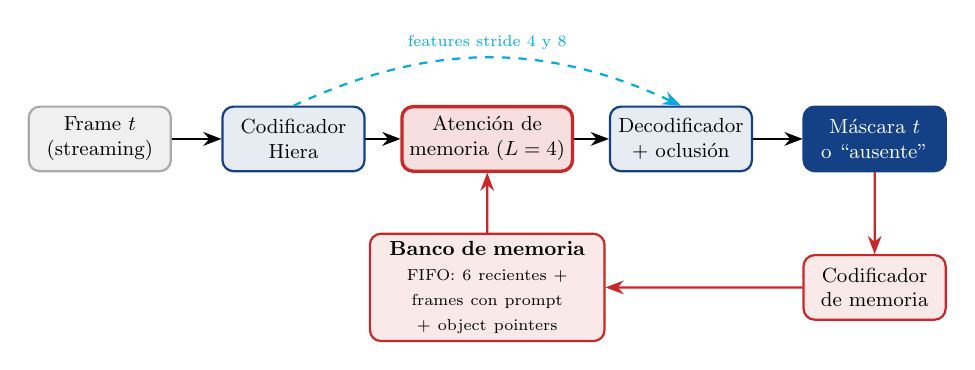
\begin{tikzpicture}[scale=0.82, every node/.style={transform shape},
				lay/.style={draw, thick, rounded corners, minimum width=2.2cm, minimum height=1.0cm, font=\small, align=center},
				arr/.style={-Stealth, thick}]
			\node[lay, draw=mitgray, fill=LightGray] (f) at (0,0) {Frame $t$\\ (streaming)};
			\node[lay, draw=FixedBlue, fill=FixedBlue!10] (h) at (3.0,0) {Codificador\\ Hiera};
			\node[lay, draw=AdaptRed, fill=AdaptRed!15, very thick] (ma) at (6.0,0) {Atenci\'on de\\ memoria ($L=4$)};
			\node[lay, draw=FixedBlue, fill=FixedBlue!10] (d) at (9.0,0) {Decodificador\\ + oclusi\'on};
			\node[lay, draw=UCMNavy, fill=UCMNavy, text=white] (m) at (12.0,0) {M\'ascara $t$\\ o ``ausente''};
			\node[lay, draw=AdaptRed, fill=AdaptRed!10, text width=3.4cm] (bank) at (6.0,-2.3) {\textbf{Banco de memoria}\\ \scriptsize FIFO: 6 recientes + frames con prompt + object pointers};
			\node[lay, draw=AdaptRed, fill=AdaptRed!10] (me) at (12.0,-2.3) {Codificador\\ de memoria};

			\draw[arr] (f) -- (h); \draw[arr] (h) -- (ma); \draw[arr] (ma) -- (d); \draw[arr] (d) -- (m);
			\draw[arr, AdaptRed] (m) -- (me);
			\draw[arr, AdaptRed] (me) -- (bank);
			\draw[arr, AdaptRed] (bank) -- (ma);
			\draw[-Stealth, dashed, UCMBlue, thick] (h.north) to[bend left=25] node[above, font=\scriptsize] {features stride 4 y 8} (d.north);
		\end{tikzpicture}
	\end{center}

	\vspace{0.1cm}

	\begin{block}{Ravi et al., Meta FAIR}
		\small
		Una imagen es un video de un solo frame: con la memoria vac\'ia, SAM 2 se comporta como SAM. Un clic de correcci\'on en cualquier frame se propaga gracias a la memoria.
	\end{block}

	\note{Del paper: la atenci\'on de memoria apila 4 bloques de self-attention y cross-attention hacia el banco. El banco es una cola FIFO con hasta 6 frames recientes y hasta M frames con prompt, m\'as object pointers. Nueva cabeza de oclusi\'on. El decodificador recibe features de alta resoluci\'on (stride 4 y 8) que se saltan la atenci\'on de memoria: relevante para objetos peque\~nos.}
\end{frame}

\begin{frame}{Lo que Aporta SAM 2, en Cifras}

	\vspace{0.2cm}

	\begin{columns}[T]
		\begin{column}{0.25\textwidth}
			\cifra{6$\times$}{m\'as r\'apido que SAM en im\'agenes y m\'as preciso: 58,9 vs 58,1 mIoU (1 clic, 23 datasets)}
		\end{column}
		\begin{column}{0.25\textwidth}
			\cifra{3$\times$}{menos interacciones que SAM + XMem++ o SAM + Cutie en video}
		\end{column}
		\begin{column}{0.25\textwidth}
			\cifra{53$\times$}{m\'as m\'ascaras que cualquier dataset VOS previo: SA-V tiene 35,5\,M en 50,9\,K videos}
		\end{column}
		\begin{column}{0.25\textwidth}
			\cifra{76,8}{$\mathcal{J}\&\mathcal{F}$ en SA-V val vs 61,4 del mejor m\'etodo previo; 43,8 FPS en una A100}
		\end{column}
	\end{columns}

	\vspace{0.3cm}

	\begin{alertblock}{Data engine}
		Con SAM 2 en el ciclo, anotar tom\'o 4,5\,s por frame frente a 37,8\,s con SAM frame a frame: $8{,}4\times$ m\'as r\'apido.
	\end{alertblock}

	\vspace{0.1cm}
	{\scriptsize Fuente: Ravi et al., \textit{SAM 2: Segment Anything in Images and Videos}, Meta FAIR. Resultados de SAM 2.1, Hiera-B+.}

	\note{Tabla 5 (6x y mIoU en SA-23), secci\'on 6.1 (3x menos interacciones), secci\'on 5.2 (53x m\'as m\'ascaras) y tabla 6 (76,8 J\&F en SA-V val contra 61,4 de SwinB-DeAOT; 43,8 FPS). La idea de anotaci\'on asistida vuelve en el caso m\'edico.}
\end{frame}

% =================================================================
\section{Aplicaciones en Oftalmolog\'ia}

\begin{frame}{De SAM a MedSAM: Cerrar la Brecha de Dominio}

	\begin{columns}[T]
		\begin{column}{0.42\textwidth}
			\begin{alertblock}{Por qu\'e SAM no basta}
				\small
				\begin{itemize}
					\item Entrenado con fotos naturales: bordes difusos y bajo contraste lo confunden.
					\item M\'ascaras sin clase: no sabe qu\'e es una hemorragia.
					\item Cada token resume $16 \times 16$ px: las lesiones diminutas se diluyen.
				\end{itemize}
			\end{alertblock}
		\end{column}

		\begin{column}{0.56\textwidth}
			\begin{block}{MedSAM (Nat.\ Commun., 2024)}
				\small
				SAM ajustado con 1.570.263 pares imagen-m\'ascara de 10 modalidades y m\'as de 30 tipos de c\'ancer. Evaluado en 86 tareas internas y 60 externas, supera a especialistas por modalidad.
			\end{block}

			\begin{block}{MedSAM2 (2025)}
				\small
				Parte de SAM 2.1; ajustado con m\'as de 455.000 pares 3D y 76.000 frames de video (TC, RM, PET, ecograf\'ia, endoscop\'ia). Reduce m\'as de 85\% el costo de anotaci\'on manual.
			\end{block}
		\end{column}
	\end{columns}

	\note{Los autores de MedSAM cuentan que SAM rend\'ia mal en im\'agenes m\'edicas porque su entrenamiento era casi solo de im\'agenes naturales. MedSAM2 lleva la idea a vol\'umenes 3D y video usando la memoria de SAM 2. Ojo: el fondo de ojo no es el foco de estos modelos; el caso de retinopat\'ia requiere adaptaciones espec\'ificas.}
\end{frame}

\begin{frame}{Retinopat\'ia Diab\'etica: el Fondo de Ojo}
	\begin{figure}
		\centering
		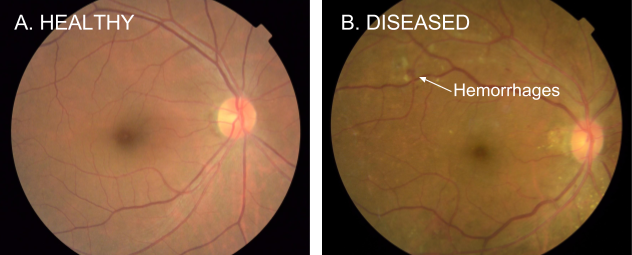
\includegraphics[width=0.8\textwidth, height=0.5\textheight,
		keepaspectratio]{figures/diabetic_eye}
	\end{figure}

	La \textbf{retinopat\'ia diab\'etica (RD)} es una de las principales causas de ceguera prevenible en adultos en edad laboral.

	\begin{columns}[T]
		\begin{column}{0.5\textwidth}
			\begin{block}{Signos visibles}
				\small
				Microaneurismas, hemorragias, exudados duros y blandos; en etapas avanzadas, neovascularizaci\'on.
			\end{block}
		\end{column}
		\begin{column}{0.5\textwidth}
			\begin{block}{Desaf\'io}
				\small
				Lesiones peque\~nas y dispersas, revisi\'on experta y cribado de poblaciones masivas.
			\end{block}
		\end{column}
	\end{columns}

	\note{Antes de las cifras epidemiol\'ogicas, mostrar c\'omo se ve una retina con RD y d\'onde aparecen las lesiones que vamos a segmentar.}
\end{frame}

\begin{frame}{Retinopat\'ia Diab\'etica en Cifras}

	\begin{columns}[T]
		\begin{column}{0.36\textwidth}
			\cifra{22,3\%}{de las personas con diabetes tiene retinopat\'ia}
			\cifra{160,5\,M}{adultos con RD proyectados para 2045}
			{\scriptsize Teo et al., \textit{Ophthalmology}, 2021.}
		\end{column}

		\begin{column}{0.62\textwidth}
			\begin{columns}[T]
				\begin{column}{0.5\textwidth}
					\begin{block}{Microaneurismas}
						\scriptsize \textbf{MA.} Dilataciones capilares; el primer signo. Miden pocos pixeles.
					\end{block}
					\begin{block}{Exudados duros}
						\scriptsize \textbf{EX.} Dep\'ositos de l\'ipidos amarillos, de bordes n\'itidos.
					\end{block}
				\end{column}
				\begin{column}{0.5\textwidth}
					\begin{block}{Hemorragias}
						\scriptsize \textbf{HE.} Sangrado intrarretiniano: manchas rojas puntiformes o en llama.
					\end{block}
					\begin{block}{Exudados blandos}
						\scriptsize \textbf{SE.} Manchas algodonosas por isquemia; blanquecinas y difusas.
					\end{block}
				\end{column}
			\end{columns}
		\end{column}
	\end{columns}

	\note{Metaan\'alisis de Teo et al. (2021): prevalencia global de RD de 22,27\% entre personas con diabetes; proyecci\'on de 160,5 millones al 2045. Un metaan\'alisis de 2024 en Eye estim\'o 1,07 millones de personas ciegas por RD en 2020. Las cuatro lesiones son las que anotan los datasets p\'ublicos a nivel de pixel.}
\end{frame}

\begin{frame}{Datos P\'ublicos con M\'ascaras por Lesi\'on}

	\begin{center}
		\footnotesize
		\begin{tabular}{>{\raggedright\arraybackslash}p{2.2cm} >{\raggedright\arraybackslash}p{2.6cm} >{\raggedright\arraybackslash}p{3.1cm} >{\raggedright\arraybackslash}p{4.9cm}}
			\toprule
			\textbf{Dataset} & \textbf{Im\'agenes con m\'ascara} & \textbf{Anotaci\'on} & \textbf{Detalle} \\
			\midrule
			IDRiD (2018) & 81 (54 entrenamiento, 27 prueba) & MA, HE, EX, SE y disco \'optico & $4288 \times 2848$ px, India; 516 im\'agenes con grado de RD y edema macular \\
			\addlinespace
			DDR & 757, de 13.673 im\'agenes & MA, HE, EX, SE & Grados de RD (escala internacional) + no gradable \\
			\addlinespace
			FGADR & 1.842 & Lesiones a nivel de pixel + grado & Incluye casos proliferativos \\
			\addlinespace
			Refined IDRiD (2026) & 81, a $1024 \times 1024$ & 7 lesiones + 4 estructuras anat\'omicas & Revisado por oftalm\'ologos; agrega neovascularizaci\'on, hemorragia v\'itrea e IRMA \\
			\bottomrule
		\end{tabular}
	\end{center}

	\begin{alertblock}{Desbalance}
		Exudados duros y hemorragias concentran la mayor\'ia de los pixeles de lesi\'on; los MA son escasos y diminutos.
	\end{alertblock}

	\note{IDRiD es el est\'andar, pero peque\~no. Su versi\'on refinada (Data, 2026) corrige errores con tres oftalm\'ologos y agrega lesiones proliferativas. DDR sirve para validar generalizaci\'on. La nota de desbalance se apoya en el dataset TJDR, donde EX y HE suman m\'as del 80\% de los pixeles de lesi\'on.}
\end{frame}

\begin{frame}{Un Flujo Base para Segmentar Lesiones}

	\vspace{0.3cm}

	\begin{center}
		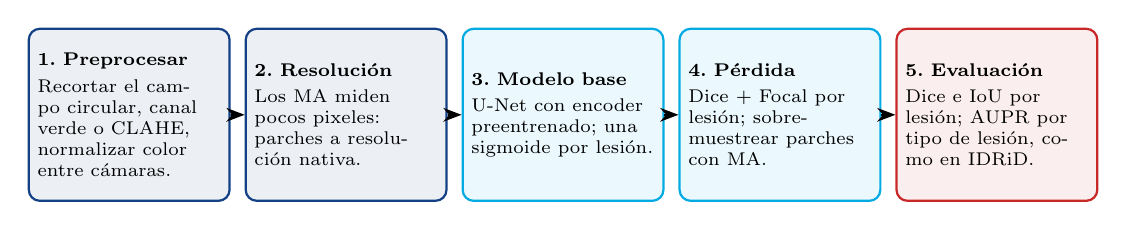
\begin{tikzpicture}[scale=0.95, every node/.style={transform shape},
				stp/.style={draw, thick, rounded corners, text width=2.45cm, minimum height=2.3cm, font=\scriptsize, align=left, anchor=north},
				arr/.style={-Stealth, thick}]
			\node[stp, draw=FixedBlue, fill=FixedBlue!8] (s1) at (0,0) {\textbf{1. Preprocesar}\\[2pt] Recortar el campo circular, canal verde o CLAHE, normalizar color entre c\'amaras.};
			\node[stp, draw=FixedBlue, fill=FixedBlue!8] (s2) at (2.9,0) {\textbf{2. Resoluci\'on}\\[2pt] Los MA miden pocos pixeles: parches a resoluci\'on nativa.};
			\node[stp, draw=UCMBlue, fill=UCMBlue!8] (s3) at (5.8,0) {\textbf{3. Modelo base}\\[2pt] U-Net con encoder preentrenado; una sigmoide por lesi\'on.};
			\node[stp, draw=UCMBlue, fill=UCMBlue!8] (s4) at (8.7,0) {\textbf{4. P\'erdida}\\[2pt] Dice + Focal por lesi\'on; sobremuestrear parches con MA.};
			\node[stp, draw=AdaptRed, fill=AdaptRed!8] (s5) at (11.6,0) {\textbf{5. Evaluaci\'on}\\[2pt] Dice e IoU por lesi\'on; AUPR por tipo de lesi\'on, como en IDRiD.};
			\foreach \a/\b in {s1/s2,s2/s3,s3/s4,s4/s5}{\draw[arr] (\a.east) -- (\b.west);}
		\end{tikzpicture}
	\end{center}

	\vspace{0.4cm}

	\begin{alertblock}{Baseline}
		Este flujo es la vara con la que se mide cualquier enfoque basado en SAM.
	\end{alertblock}

	\note{El canal verde concentra el contraste de lesiones rojas y amarillas. Reducir una imagen de 4288 px de ancho a 512 px puede borrar por completo un microaneurisma. Salida multietiqueta porque las lesiones pueden superponerse.}
\end{frame}

\begin{frame}{Tres Maneras de Usar SAM en el Fondo de Ojo}

	\begin{columns}[T]
		\begin{column}{0.33\textwidth}
			\begin{block}{1. Prompts desde la mirada}
				\small
				\textit{GlanceSeg (Jiang et al.)}

				\vspace{0.1cm}
				El mapa de mirada del oftalm\'ologo ubica la zona; un mapa de saliencia genera puntos-prompt para SAM y un filtro de conocimiento m\'edico depura los MA, en tiempo real.
			\end{block}
		\end{column}

		\begin{column}{0.33\textwidth}
			\begin{block}{2. Ajuste eficiente + texto}
				\small
				\textit{TP-DRSeg (MICCAI 2024)}

				\vspace{0.1cm}
				Describe cada lesi\'on con texto expl\'icito y lo inyecta en el codificador de SAM con ajuste eficiente de par\'ametros. Obtiene m\'ascaras con clase.
			\end{block}
		\end{column}

		\begin{column}{0.33\textwidth}
			\begin{block}{3. Anotaci\'on asistida}
				\small
				\textit{Idea del data engine de SAM 2}

				\vspace{0.1cm}
				SAM o MedSAM aceleran el etiquetado y el experto corrige. Las m\'ascaras entrenan un U-Net especializado y barato de ejecutar.
			\end{block}
		\end{column}
	\end{columns}

	\note{GlanceSeg resuelve el problema del prompt usando seguimiento ocular. TP-DRSeg ataca que SAM produce m\'ascaras sin clase y le cuesta distinguir lesiones parecidas; evaluado en IDRiD y DDR. La tercera estrategia es la m\'as pragm\'atica hoy en un hospital: el modelo fundacional como herramienta de anotaci\'on, no como modelo final.}
\end{frame}

\begin{frame}{Desaf\'ios Abiertos}

	\begin{columns}[T]
		\begin{column}{0.5\textwidth}
			\begin{block}{Lesiones diminutas}
				\small
				Embedding de $64 \times 64$: cada token cubre $16 \times 16$ px. SAM 2 suma features de stride 4 y 8 al decoder, pero los MA siguen al l\'imite.
			\end{block}
			\begin{block}{Desbalance extremo}
				\small
				Casi todo es fondo: Dice y Focal ayudan; evaluar por tipo de lesi\'on.
			\end{block}
			\begin{block}{Cambio de dominio}
				\small
				C\'amaras, poblaciones y protocolos distintos: validar siempre en un dataset externo.
			\end{block}
		\end{column}

		\begin{column}{0.5\textwidth}
			\begin{block}{Calidad del ground truth}
				\small
				Bordes difusos en exudados blandos y hemorragias. En IDRiD las m\'ascaras las traz\'o un estudiante entrenado por oftalm\'ologos; la versi\'on refinada corrige errores.
			\end{block}
			\begin{alertblock}{Del pixel a la decisi\'on cl\'inica}
				\small
				La m\'ascara debe traducirse en un grado de RD y una derivaci\'on, con validaci\'on prospectiva y aprobaci\'on regulatoria.
			\end{alertblock}
		\end{column}
	\end{columns}

	\note{Pregunta para discusi\'on: si SAM 2 ya incorpora features de alta resoluci\'on, ?`qu\'e cambios har\'ian falta para que un microaneurisma de 5 a 10 pixeles sea segmentable? Posibles respuestas: recortes ampliados, prompts m\'as densos, o ajustar el decodificador con datos de fondo de ojo.}
\end{frame}

\begin{frame}{Actividad Pr\'actica: U-Net vs.\ SAM en IDRiD}

	\begin{enumerate}
		\item Entrenar un U-Net para \textbf{exudados duros}, primero con BCE y luego con Dice + Focal. Comparar Dice y AUPR en las 27 im\'agenes de prueba.
		      \vspace{0.25cm}
		\item Evaluar \textbf{SAM o MedSAM} sin ajuste, con cajas derivadas del ground truth y con 1, 3 y 5 clics por lesi\'on.
		      \vspace{0.25cm}
		\item Discutir: ?`cu\'antos clics necesita SAM para igualar al U-Net? ?`En qu\'e lesiones falla y por qu\'e?
	\end{enumerate}

	\vspace{0.3cm}

	\begin{block}{Entregable}
		Notebook \texttt{labs/2.6.2\_SegmentacionRetinopatiaSAM.ipynb} + informe breve con una tabla de m\'etricas por lesi\'on y m\'etodo.
	\end{block}

	\note{El paso 2 replica el protocolo del paper de SAM: primer clic en el centro de la lesi\'on, los siguientes en el centro de la regi\'on de error. Empezar con exudados duros, la clase m\'as abundante, antes de intentar microaneurismas.}
\end{frame}

% =================================================================
\section{Resumen}

\begin{frame}{Conclusiones}

	\begin{itemize}
		\item \textbf{Fundamentos:} segmentar es clasificar cada pixel; medir con Dice e IoU, nunca solo exactitud.

		\vspace{0.25cm}

		\item \textbf{Arquitecturas:} U-Net (datos peque\~nos), DeepLab (contexto multiescala), transformers (clasificaci\'on de m\'ascaras).

		\vspace{0.25cm}

		\item \textbf{Funciones objetivo:} combinar CE o Focal + Dice; Tversky si la sensibilidad manda.

		\vspace{0.25cm}

		\item \textbf{SAM / SAM 2:} segmentaci\'on por prompts sin clases; SAM 2 agrega memoria para video.

		\vspace{0.25cm}

		\item \textbf{Retinopat\'ia diab\'etica:} lesiones diminutas y desbalanceadas; SAM sirve mejor adaptado o como herramienta de anotaci\'on.
	\end{itemize}

\end{frame}

\begin{frame}{Referencias}

	\begin{columns}[T]
		\begin{column}{0.5\textwidth}
			\textbf{\small Arquitecturas y p\'erdidas}
			\vspace{0.1cm}

			\scriptsize
			Long et al. (2015). FCN. \textit{CVPR}.\\
			Ronneberger et al. (2015). U-Net. \textit{MICCAI}.\\
			Badrinarayanan et al. (2017). SegNet. \textit{TPAMI}.\\
			Milletari et al. (2016). V-Net (Dice loss). \textit{3DV}.\\
			Zhao et al. (2017). PSPNet. \textit{CVPR}.\\
			He et al. (2017). Mask R-CNN. \textit{ICCV}.\\
			Lin et al. (2017). Focal loss. \textit{ICCV}.\\
			Salehi et al. (2017). Tversky loss. \textit{MLMI}.\\
			Chen et al. (2018). DeepLabv3+. \textit{ECCV}.\\
			Berman et al. (2018). Lov\'asz-Softmax. \textit{CVPR}.\\
			Kervadec et al. (2019). Boundary loss. \textit{MIDL}.\\
			Xie et al. (2021). SegFormer. \textit{NeurIPS}.\\
			Cheng et al. (2022). Mask2Former. \textit{CVPR}.
		\end{column}

		\begin{column}{0.5\textwidth}
			\textbf{\small SAM y medicina}
			\vspace{0.1cm}

			\scriptsize
			Kirillov et al. (2023). Segment Anything. \textit{ICCV}.\\
			Ravi et al. (2025). SAM 2. \textit{ICLR}.\\
			Ma et al. (2024). MedSAM. \textit{Nat. Commun.} 15:654.\\
			Ma et al. (2025). MedSAM2. arXiv:2504.03600.\\
			Teo et al. (2021). Prevalencia global de RD. \textit{Ophthalmology}.\\
			Porwal et al. (2018). IDRiD. \textit{Data} 3(3):25.\\
			Li et al. (2019). DDR. \textit{Information Sciences}.\\
			Jiang et al. (2023). GlanceSeg. arXiv:2311.08075.\\
			TP-DRSeg (2024). \textit{MICCAI}. github.com/wxliii/TP-DRSeg
		\end{column}
	\end{columns}

\end{frame}

\end{document}
